\section{Case-study : deploying a machine learning model in production following MLOps principles}
\label{sec:mlops}

This chapter aims, through a concrete example, to illustrate how Insee managed to deploy its first machine learning (ML) model into production. It will delve into the MLOps approach that this project strived to adhere to as much as possible, focusing on the various technologies that were employed. In particular, we will highlight how cloud technologies were instrumental in building a solution iteratively and how Onyxia greatly facilitated this process by providing flexible development environments. The entire project is available in open source\footnote{\url{https://github.com/orgs/InseeFrLab/teams/codification-ape/repositories}} and remains under active development.

\subsection{Motivation}

Coding tasks are common operations for NSOs and can sometimes be challenging due to the size of nomenclatures. At Insee, a sophisticated coding tool called Sicore was developed in the 1990s to perform various classification tasks. It consists in a coding engine containing a large number of deterministic rules which identify ground-truth labels. Each input label goes through these rules and when a ground-truth label is recognized, the associated code is assigned. When the label is not recognized, it must be manually classified by an Insee agent. 

Two main reasons drove the experimentation of new coding methods. Firstly, there was an internal change with the redesign of the Sirene registry, which lists all companies in France and assigns them a unique identifier, the Siren number, used by public institutions. The main goals of this revamping were to improve the daily management of the registry for Insee agents and to reduce waiting times for companies. Additionally, at the national level, the government launched a one-stop shop for business formalities, allowing more flexibility for business owners in describing their main activities. Initial testing exercises revealed that Sicore was no longer the suitable tool for performing NACE classification, as only 30\% of the input data were being automatically coded.

Three stakeholders were involved in this project: the \textit{business team}\footnote{We refer to the business team, the team that has business knowledge i.e. who knows the NACE perfectly.} responsible for managing the Sirene registry, the \textit{IT team} developing software related to the registry's operation, and the \textit{innovation team} responsible for implementing the new coding tool. The latter team is the Insee Lab, which was created in 2017 with the objective of providing support to other teams on innovation topics to streamline their various projects.

\subsection{Project details}

The project we are describing is a standard NLP classification problem. Starting from a textual description of the activity, we want to predict the associated class in the NACE Rev. 2 nomenclature. This nomenclature has the particularity of being hierarchical and contains 5 different levels\footnote{Actually, there are 5 different levels in France but only 4 at the European level.}: section, division, group, class, and subclass. In total, 732 subclasses are included in the nomenclature, which is the level at which we aim to perform the classification. Table \ref{tab:nace-nomenclature} provides an example of this hierarchical structure.

\begin{table}[htbp]
    \centering
    \begin{tabular}{llll}
    \textbf{Level} & \textbf{NACE} & \textbf{Title} & \textbf{Size} \\ \hline
    Section & H & Transportation and storage & 21 \\ \hline
    Division & 52 & Warehousing and support activities for transportation & 88 \\ \hline
    Group & 522 & Support activities for transportation & 272 \\ \hline
    Class & 5224 & Cargo handling & 615 \\ \hline
    \textbf{Subclass} & \textbf{\textcolor{red}{5224A}} & \textbf{Harbour handling} & \textbf{\textcolor{red}{732}} \\ 
    \end{tabular}
    \caption{NACE Nomenclature}
    \label{tab:nace-nomenclature}
    \end{table}

With the establishment of the one-stop shop, business owners now describe their activity description with a free-text field. As a result, the new labels are very different from the harmonized labels that were previously received. Therefore, it was decided to work with ML models, as they have proven their effectiveness on such tasks in the literature. This represents a significant paradigm shift from Insee's perspective, as ML was not traditionally used in the actual production of official statistics. Besides, the perspective of putting the new model in production was considered from the outset, guiding numerous methodological and technical choices. As such, several points had to be agreed upon to facilitate coordination among the various stakeholders, and several strategic choices had to be made from the outset, including the methodology, the choice of a development environment, and collaborative work methods.

\subsubsection{Methodology}

When it came to selecting the methodology to adopt, we had to navigate through various constraints, with the most significant being the need for deployment on our production servers. Our model had to be lightweight enough to run efficiently on these servers, while also minimizing the computational resource overhead to ensure swift inference. Additionally, the model had to be compatible with a different language than the one it was trained, namely Java, utilized on our production servers. This proved particularly challenging throughout our project, as it influenced our data preprocessing choices, necessitating simplicity wherever possible. We had to meticulously replicate the data processing performed in Python during training, thereby limiting the use of certain packages. Ultimately, each decision made had to ensure the model's compatibility and efficiency within a production environment while minimizing compromises on inference quality.

These constraints led us away from the most powerful language models at the start of the project, such as Transformer models, and instead directed us towards simpler natural language models. Specifically, we opted for the fastText model \cite{joulin2016bag}. This choice was driven by its ability to address all previously mentioned constraints. The fastText model is incredibly fast to train, even from scratch, and inference doesn't require a GPU to be extremely rapid. Moreover, there exists a wrapper that enables reading fastText models in Java, which could be utilized by the IT teams on their machines, greatly facilitating the deployment of our models. Unfortunately, this wrapper, available on \href{https://github.com/vinhkhuc/JFastText}{GitHub}, is no longer maintained, posing serious security concerns, and thus became a temporary default choice for us. In addition to these technical arguments, the decision to use the fastText model was justified from a methodological standpoint. Firstly, the Insee Lab teams had already completed several projects using the fastText model, leveraging the acquired knowledge to achieve initial results very quickly. While it may not have been a state-of-the-art language model, for our use case, the model yielded excellent performance results which, considering the time and human resource constraints, were more than sufficient to enhance the existing process. Finally, the model is inherently simple methodologically speaking, greatly simplifying communication and adoption within the various Insee teams. 

The supervised classification model fastText relies on both a bag-of-words model to obtain embeddings and a classifier based on logistic regression. The bag-of-words approach involves representing a text as the set of vector representations of each of its constituent words. Thus, the embedding of a sentence depends on the embeddings of its words, for example, their sum or their average. In the case of supervised text classification, the embedding matrix and the classifier's coefficient matrix are learned simultaneously during training by gradient descent, minimizing an usual cross-entropy loss function. The specificity of the fastText model lies in embeddings being performed not only on words but also on word n-grams and character n-grams, providing more context and reducing biases due to spelling mistakes. The fastText model can be summarized by the Figure \ref{fig:fasttext}

\begin{figure}[htbp]
    \centering
    \makebox[\textwidth][c]{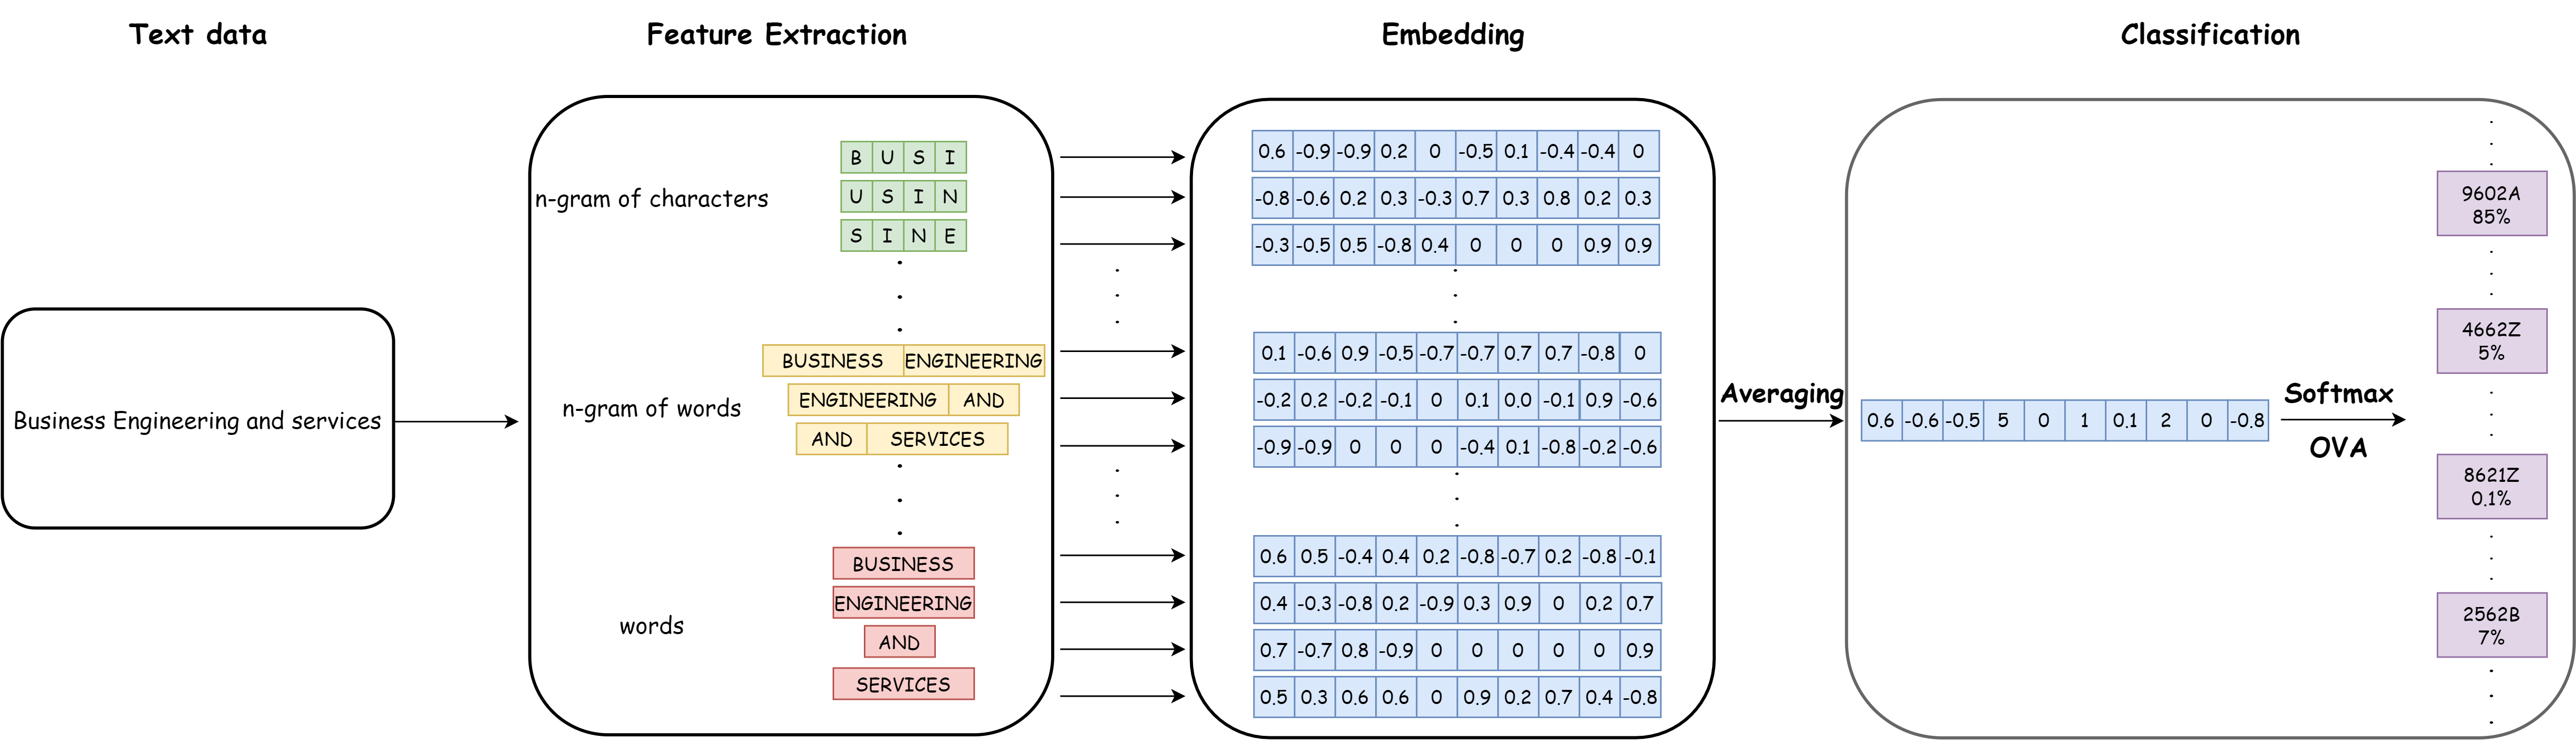
\includegraphics[width=1.5\textwidth]{sections/img/fasttext.png}}
    \caption{Simplified architecture of the fastText model}
    \label{fig:fasttext}
\end{figure}

\subsubsection{Development environment}

In a ML project, the choice of a flexible development infrastructure is paramount. First, due to the diversity of tasks to be performed — data collection, preprocessing, modeling, evaluation, inference, monitoring, etc. Second, because machine learning is a fast-evolving field. It is thus preferable to build a ML app as a collection of modular components so as to be able to update components without disrupting the entire pipeline. In order to leverage the flexibility of cloud technologies, the Onyxia project — and in particular its open-innovation instance, the SSP Cloud — was chosen as the main development environment. This projects also illustrates the richness of Onyxia's catalog of services, as we used a variety of tools for each stage of our pipeline: MinIO, Vault, MLflow, ArgoCD, Argo Workflows, Label Studio. The decision to opt for the SSP Cloud was also motivated by the ongoing implementation of a private instance of Onyxia on the production servers at Insee. This initiative is poised to streamline the connection between production and development environments in the long run. Finally, this project relied exclusively on open-data and thus complied with the open policy of the SSP Cloud.

\subsubsection{Enforcing best development practices}

From the very onset of this project, the target was to go beyond mere experimentation and put the model in production as soon as possible. Consequently, we strived to enforce best development practices from the very beginning of the project. All the development was versioned with Git and put in open-source on GitHub\footnote{\url{https://github.com/orgs/InseeFrLab/teams/codification-ape/repositories}}. In terms of code quality, we tried to comply to community standards, e.g. using formatters such as \href{https://github.com/astral-sh/ruff}{Ruff}. Scripts were favored over notebooks in order to favor a modular package-like structure for the project which is much better suited to the integration into automated data transformation and ML pipelines.



\subsection{What is MLOps?}


\subsubsection{Specificities of ML projects}

In the landscape of ML projects, there are new considerations and challenges compared to traditional statistical projects. These new challenges stem from the complex nature of ML models, their iterative development process, and the need for automation and scalability. Among others, here are some key aspects in ML projects:

\begin{enumerate}
    \item \textbf{Logging Parameters}: ML models often have numerous hyperparameters and configurations that significantly impact their performance. It's crucial to log these parameters along with model training and evaluation metrics to ensure reproducibility and traceability. This logging allows for better understanding of model behavior and facilitates debugging and optimization efforts.
    
    \item \textbf{Optimizing Hyperparameters}: Tuning hyperparameters is a critical step in optimizing the performance of ML models. Unlike traditional statistical models where parameters are often predefined, ML models typically have a larger number of hyperparameters that need to be optimized. This process requires sophisticated techniques such as grid search, random search, or Bayesian optimization, which can be computationally intensive and time-consuming.
    
    \item \textbf{Model Versioning}: ML models are highly iterative. Therefore, effective version control mechanisms are essential to track changes, compare performance across different model versions, and roll back to previous versions if necessary. While model versioning may also be relevant for traditional statistical models, it is infrequently practiced. In ML projects, however, it is considered mandatory due to the iterative nature of model development and the dynamic nature of data and algorithms.
    
    \item \textbf{Model Deployment}: Deploying ML models into production environments presents unique challenges due to their complexity and resource requirements. Ensuring seamless deployment involves considerations such as containerization, scalability, latency, and harmonization with preexisting systems.
    
    \item \textbf{Model Monitoring}: Once deployed, ML models need to be continuously monitored to detect performance degradation, concept drift, or other anomalies. Unlike traditional statistical models, ML models can exhibit unexpected behavior over time due to changes in data distribution or underlying patterns. Implementing robust monitoring solutions involves tracking model performance metrics and data quality to ensure ongoing reliability, effectiveness and to trigger model retraining.

    \item \textbf{Model Retraining}: Regular retraining of ML models stands as an imperative to maintain their effectiveness over time. Shifts in data distribution, variations in data quality, or evolving business imperatives may necessitate the recalibration of models to preserve accuracy and relevance. 

    \item \textbf{Data Annotation}: The process of data annotation assumes paramount importance in the context of ML, where labeled datasets serve as the foundation for model training and validation. Data annotation involves the manual or automated labeling of raw data with descriptive metadata, facilitating the development of supervised learning models. Data annotation directly influences the performance and generalizability of ML models.

    \item \textbf{Explainability}: The interpretability of ML models is important for building trust and understanding their predictions.
\end{enumerate}


\subsubsection{From DevOps to MLOps}

The MLOps approach is built upon the foundations of the DevOps approach. In this sense, it can be considered simply as an extension of DevOps, developed to address the specific challenges related to managing the lifecycle of ML models. MLOps incorporates the principles of collaboration and automation inherent in DevOps but also considers all aspects related to data and ML models.

\begin{figure}[htbp]
    \centering
    \makebox[\textwidth][c]{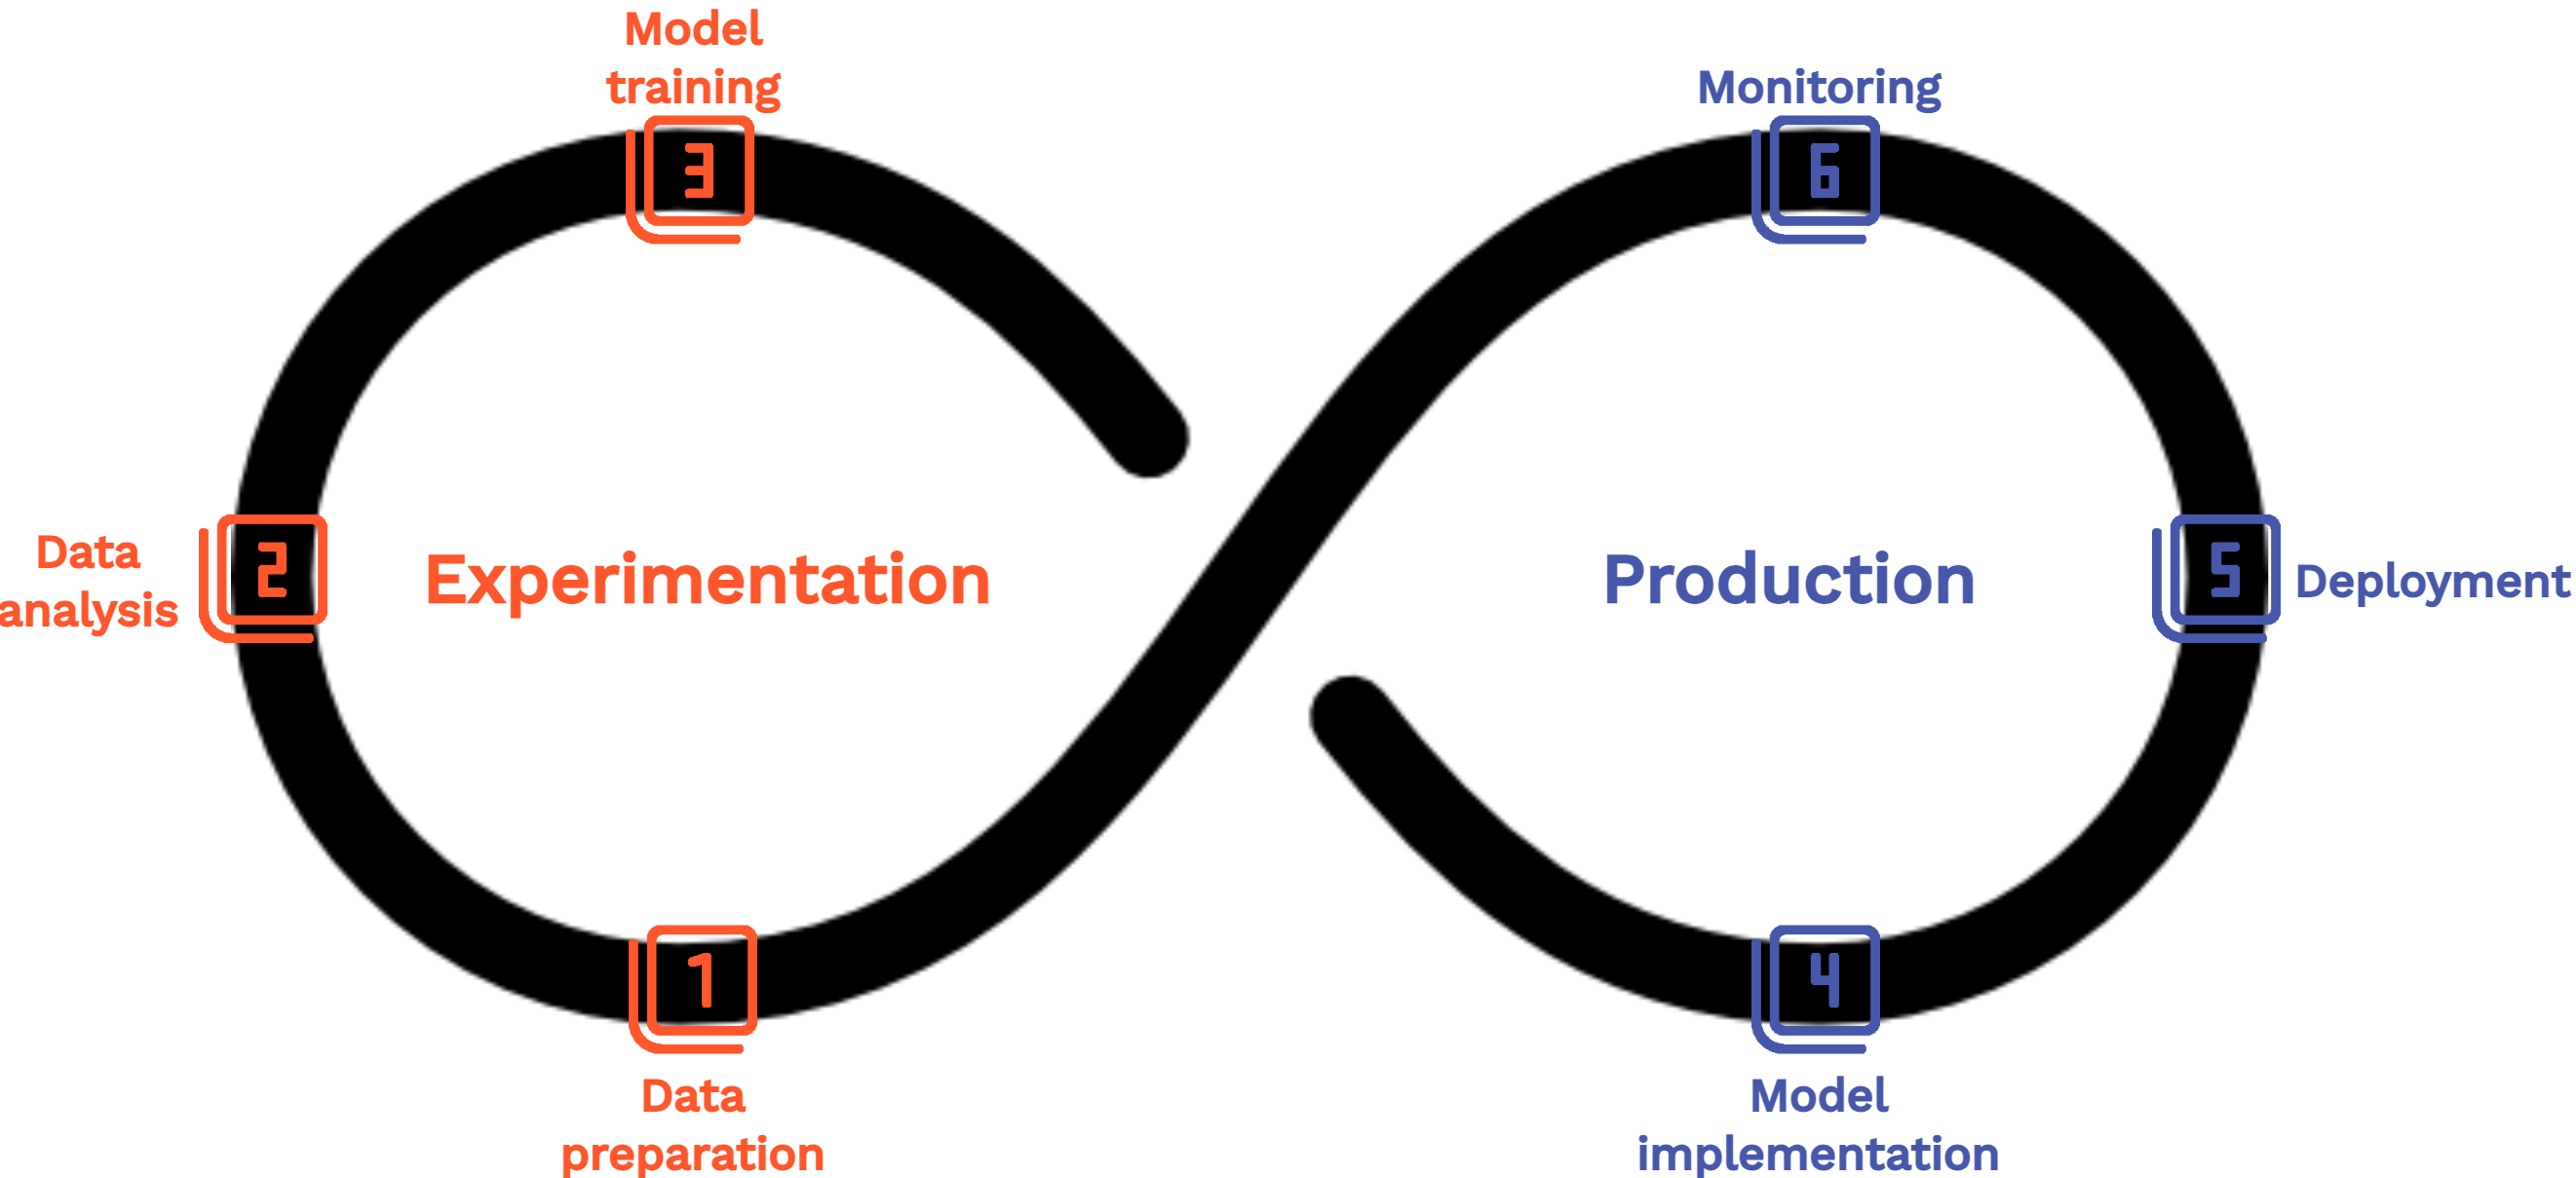
\includegraphics[width=\textwidth]{sections/img/mlops-cycle.png}}
    \caption{Machine Learning lifecycle. Credits: Satish Chandra Gupta}
    \label{fig:mlops-cycle}
\end{figure}


MLOps involves the automation of tasks such as data management, tracking model versions, their deployments, as well as the continuous evaluation of model performance in production. Similar to DevOps, MLOps emphasizes close collaboration between business units and IT teams on one hand, and data science teams on the other. This collaboration is key to ensuring effective communication throughout the lifecycle of the ML model.

\subsubsection{MLOps Principles}

The pillars of MLOps\cite{kreuzberger2023machine} are generally defined as :

\begin{itemize}
    \item \textbf{Reproducibility}: The results of every experiment, successful or unsuccessful, should be reproducible at no cost. This implies first and foremost a certain rigor in managing packages, environments, system libraries, code version control, etc. Additionally, the various variables influencing model training (training data, hyperparameters, etc.) must be versioned with the model.
    
    \item \textbf{Automation}: To foster feedback loops of continuous improvement, the model lifecycle (testing, building, validation, deployment) must be automated to the fullest extent possible. Tools derived from the DevOps approach, especially continuous integration and continuous deployment (CI/CD), should be leveraged.
    
    \item \textbf{Collaboration}: MLOps values a culture of collaborative work around ML projects, where communication within teams should reduce siloed work. On a technical level, MLOps tools used should facilitate collaborative work on data, model, and code used by the project.
    
    \item \textbf{Continuous Improvement}: Once deployed, it is essential to ensure that the model performs as expected by evaluating its performance on real data using continuous monitoring tools. In case of performance degradation over time, periodic retraining or continuous training of the model should be considered.
\end{itemize}


Tackling these challenges and effectively managing the lifecycle of a ML project necessitates specialized tools, many of which are accessible as open-source solutions. Throughout our project, we aimed to embrace the MLOps approach by utilizing software applications grounded in cloud-native technologies and available in the SSP Cloud catalog. This enables data scientists to be autonomous from model training to deployment.

\subsection{MLflow as the cornerstone of the project}

During this project, we heavily relied on \href{https://github.com/MLflow/MLflow}{MLflow}, a platform designed to streamline the lifecycle of ML models. It allows for detailed tracking of various experiments, packaging of code to ensure reproducibility, and serving models to end-users. MLflow also features an API that is compatible with most ML libraries such as PyTorch, Scikit-learn, XGBoost, and supports multiple programming languages including Python, R, and Java. It incorporates various functionalities that facilitate the adoption of the MLOps approach.

There are numerous tools available for orchestrating tasks and data pipelines. Among the most popular (based on their GitHub stars) are \href{https://github.com/apache/airflow}{Airflow}, \href{https://github.com/spotify/luigi}{Luigi}, \href{https://github.com/argoproj/argo-workflows}{Argo Workflows}, \href{https://github.com/PrefectHQ/prefect}{Prefect}, \href{https://github.com/kubeflow/kubeflow}{Kubeflow} and \href{https://github.com/bentoml/BentoML}{BentoML}. It's difficult to assert whether one is better to another; in reality, your choice largely depends on your IT infrastructure and project requirements. In our case, we opted to use MLflow for its ease of use and suitability for ML projects. Additionally, it is available in the SSP Cloud catalog, simplifying its installation process and its connection with our MinIO storage where all the artifacts are automatically stored.

\subsubsection{MLflow Projects}

MLflow offers a format for packaging data science projects to promote code reuse and reproducibility. This format is simply called \href{https://MLflow.org/docs/latest/projects.html}{MLflow Project}. Essentially, an MLflow project is nothing more than a directory containing the code and necessary resources (data, configuration files, etc.) for executing your project. It is summarized by an `MLproject` file listing the various commands to execute a pipeline as well as the necessary dependencies. In general, an MLflow project has the following structure:

\dirtree{%
.1 Project\_ML/.
.2 artifacts/.
.3 model.bin.
.3 train\_text.txt.
.2 code/.
.3 main.py.
.3 preprocessing.py.
.2 MLmodel.
.2 conda.yaml.
.2 python\_env.yaml.
.2 python\_model.pkl.
.2 requirements.txt.
}


\subsubsection{MLflow Models}

In addition to packaging a project, MLflow also allows you to package your model, regardless of the underlying ML library used\footnote{You also have the capability to package our own custom model. This is precisely what we do to integrate our fastText model into MLflow.}  (among those \href{https://MLflow.org/docs/latest/models.html#built-in-model-flavors}{compatible with MLflow}, i.e., all the libraries you use!). Thus, two models trained with different libraries, say PyTorch and Keras, can be deployed and queried in the same way thanks to this layer added by MLflow. This harmonization becomes particularly valuable as you begin to accumulate various types of models, as it eliminates the need to modify your inference pipeline every time you introduce a new model type.

\subsubsection{Tracking Server}

MLflow provides a tracking server that includes both an ergonomic graphical interface and an API for logging various parameters, metrics, files, etc. during the training of your ML model. The tracking server is very useful for comparing the different experiments you have performed, storing them, and also being able to reproduce them. Indeed, each run stores the source of the utilized data along with the corresponding commit. When combined with MLflow Project, this capability enables the reproduction of every conducted run.

\subsubsection{Model Registry}

Once different experiments have been conducted and models that satisfy us have been selected, it is time to move on to the next step in the model lifecycle. Indeed, the chosen model must then be able to move into a production or pre-production environment. However, knowing the state of a model in its lifecycle requires very rigorous organization and is not so straightforward. MLflow has developed a feature that simplifies this version management of models through its \href{https://MLflow.org/docs/latest/model-registry.html}{Model Registry}. This registry allows you to add tags and aliases to your models to define their position in their lifecycle and thus be able to retrieve them efficiently.

In general, a ML model goes through 4 stages that need to be known at all times:

\begin{enumerate}
    \item \textbf{Experimental}
    \item \textbf{Staging}
    \item \textbf{Production}
    \item \textbf{Archived}
\end{enumerate}


\subsubsection{MLflow in short}

MLflow is an open-source project that provides a platform for tracking the lifecycle of a ML model from start to finish. It is not the only available tool, and it may not be the most suitable for some of your specific projects. However, we believe it offers several advantages, primarily its ease of use and its ability to meet the needs of the MLOps approach. It is important to keep in mind that this environment is still very new, and new open-source projects emerge every day, so it is necessary to stay up to date on the latest developments. In summary, MLflow allows you to:

\begin{itemize}
    \item Simplify tracking the training of ML models through its API and tracking server.
    \item Integrate the main ML frameworks easily.
    \item Integrate your own framework if needed.
    \item Standardize your training script, enabling industrialization, for example, fine-tuning hyperparameters.
    \item Package your models for easy and harmonized querying across different frameworks.
    \item Store your models efficiently by assigning tags and facilitating lifecycle tracking.
\end{itemize}

\begin{figure}[htbp]
    \centering
    \makebox[\textwidth][c]{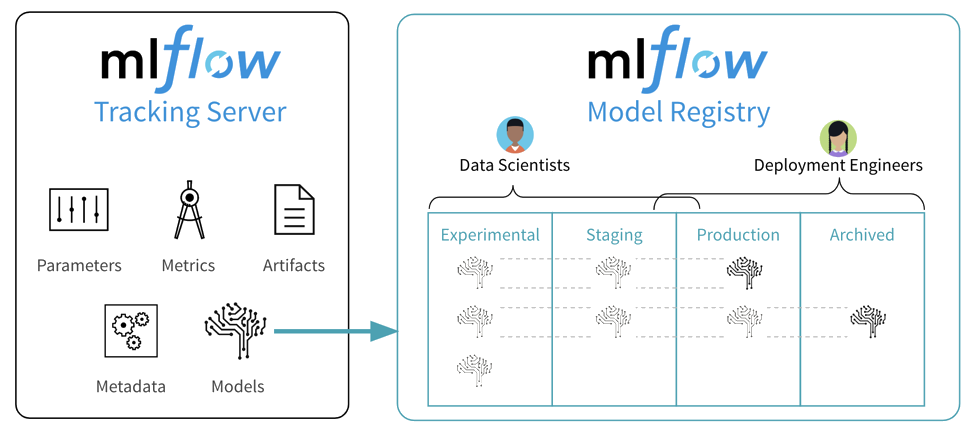
\includegraphics[width=\textwidth]{sections/img/mlflow-model-registry.png}}
    \caption{TODO}
    \label{fig:mlflow-registry}
\end{figure}


\subsection{Embracing the potential of Onyxia from training to deployment}

To adhere closely to the MLOps approach, we strived to automate as much as possible the various stages of the ML model lifecycle. In the "automation" section of the SSP Cloud \href{https://datalab.sspcloud.fr/catalog/automation}{catalog}, several services are available in addition to MLflow, including Argo CD and Argo Workflows, which we use in a daily basis for various applications.

Argo Workflows is an open-source container-native workflow engine designed for orchestrating parallel jobs on Kubernetes. It allows users to define complex multi-step workflows as code using YAML or JSON, simplifying the automation and management of tasks in a Kubernetes environment. The idea is to define workflows where each step of the process is a completely isolated container to ensure reproducibility. This allows for easy parallel execution of compute-intensive tasks for model training or data processing. In our case, we use it during the model training phase, particularly to optimize the various hyperparameters of our models. Instead of performing a grid search that would test all possible combinations in a single container, Argo Workflows creates as many containers as there are model combinations to train, with each container handling the training of a single model. Kubernetes optimizes resources within the cluster, and since we have configured MLflow in our code, all models and their metrics appear on the Tracking Server. It then becomes straightforward to compare the different trained models and select the best one using the comparison and visualization tools available on the UI. 

It is worth noting that it is relatively simple to make all these applications (Argo Workflows, MLflow, MinIO) communicate with each other with just a few configuration files because everything is well set up initially thanks to the Onyxia software. Without Onyxia, even the installation of these softwares would have been challenging.

The use of tools like Argo Workflows is highly recommended for ML projects, firstly because they rely on technologies that promote reproducibility (containers), but also because they encourage viewing projects as a series of independent steps ranging from data retrieval to result dissemination via modeling. Adopting a pipeline-based approach to your ML or statistics projects is the first step toward greater reproducibility.

% \subsubsection{Making your model accessible with SSP Cloud}

Once you have optimized, evaluated, and selected your best-performing model, it's crucial to make it available to other users. Unfortunately, this aspect is often overlooked by data scientists. A trivial way to share the model would be to provide your code and all necessary information to a third party to retrain your model on their own. Obviously, this approach is not optimal as it assumes that all users have the resources, infrastructure, and knowledge required for training. The goal is therefore to make your model available in a simple and efficient manner. The use of the SSP Cloud platform greatly simplifies this process and has also allowed us, as data scientists, to take control of our model until its deployment without relying on the IT team. Indeed, on the platform, it is possible to open services with Kubernetes administrator rights, enabling the deployment of applications. For making our ML model available, we opted to use a REST API. This seems to be the most suitable method in the vast majority of cases, as it meets several criteria:

\begin{itemize}
    \item \textbf{Simplicity}: REST APIs provide an entry point that can hide the underlying complexity of the model, making its availability easier.
    \item \textbf{Standardization}: One of the main advantages of REST APIs is that they are based on the HTTP standard. This means they are language-agnostic, and requests can be made in XML, JSON, HTML, etc.
    \item \textbf{Modularity}: The client and server are independent. In other words, data storage, user interface, or model management are completely separated from the server.
    \item \textbf{Scalability}: The separation between the server and client allows REST APIs to be highly flexible and facilitate scalability. They can adapt to the load of concurrent requests.
\end{itemize}

To develop our API, we used the popular Python library FastAPI, which is relatively easy to use and comes with exhaustive \href{https://fastapi.tiangolo.com/}{documentation}. The idea is to encapsulate all the API code and required software dependencies into a Docker image so that it can be deployed in a container on the Kubernetes cluster. Upon startup, the API will automatically retrieve the correct model from the MLflow model registry, which is located in a MinIO bucket. Using a MLflow model allows automatic integration of preprocessing before each prediction, regardless of the model framework used, greatly simplifying inference and ensuring streamlined code in the API. The model deployment process is summarized in Figure \ref{fig:api-datalab}.

\begin{figure}[htbp]
    \centering
    \makebox[\textwidth][c]{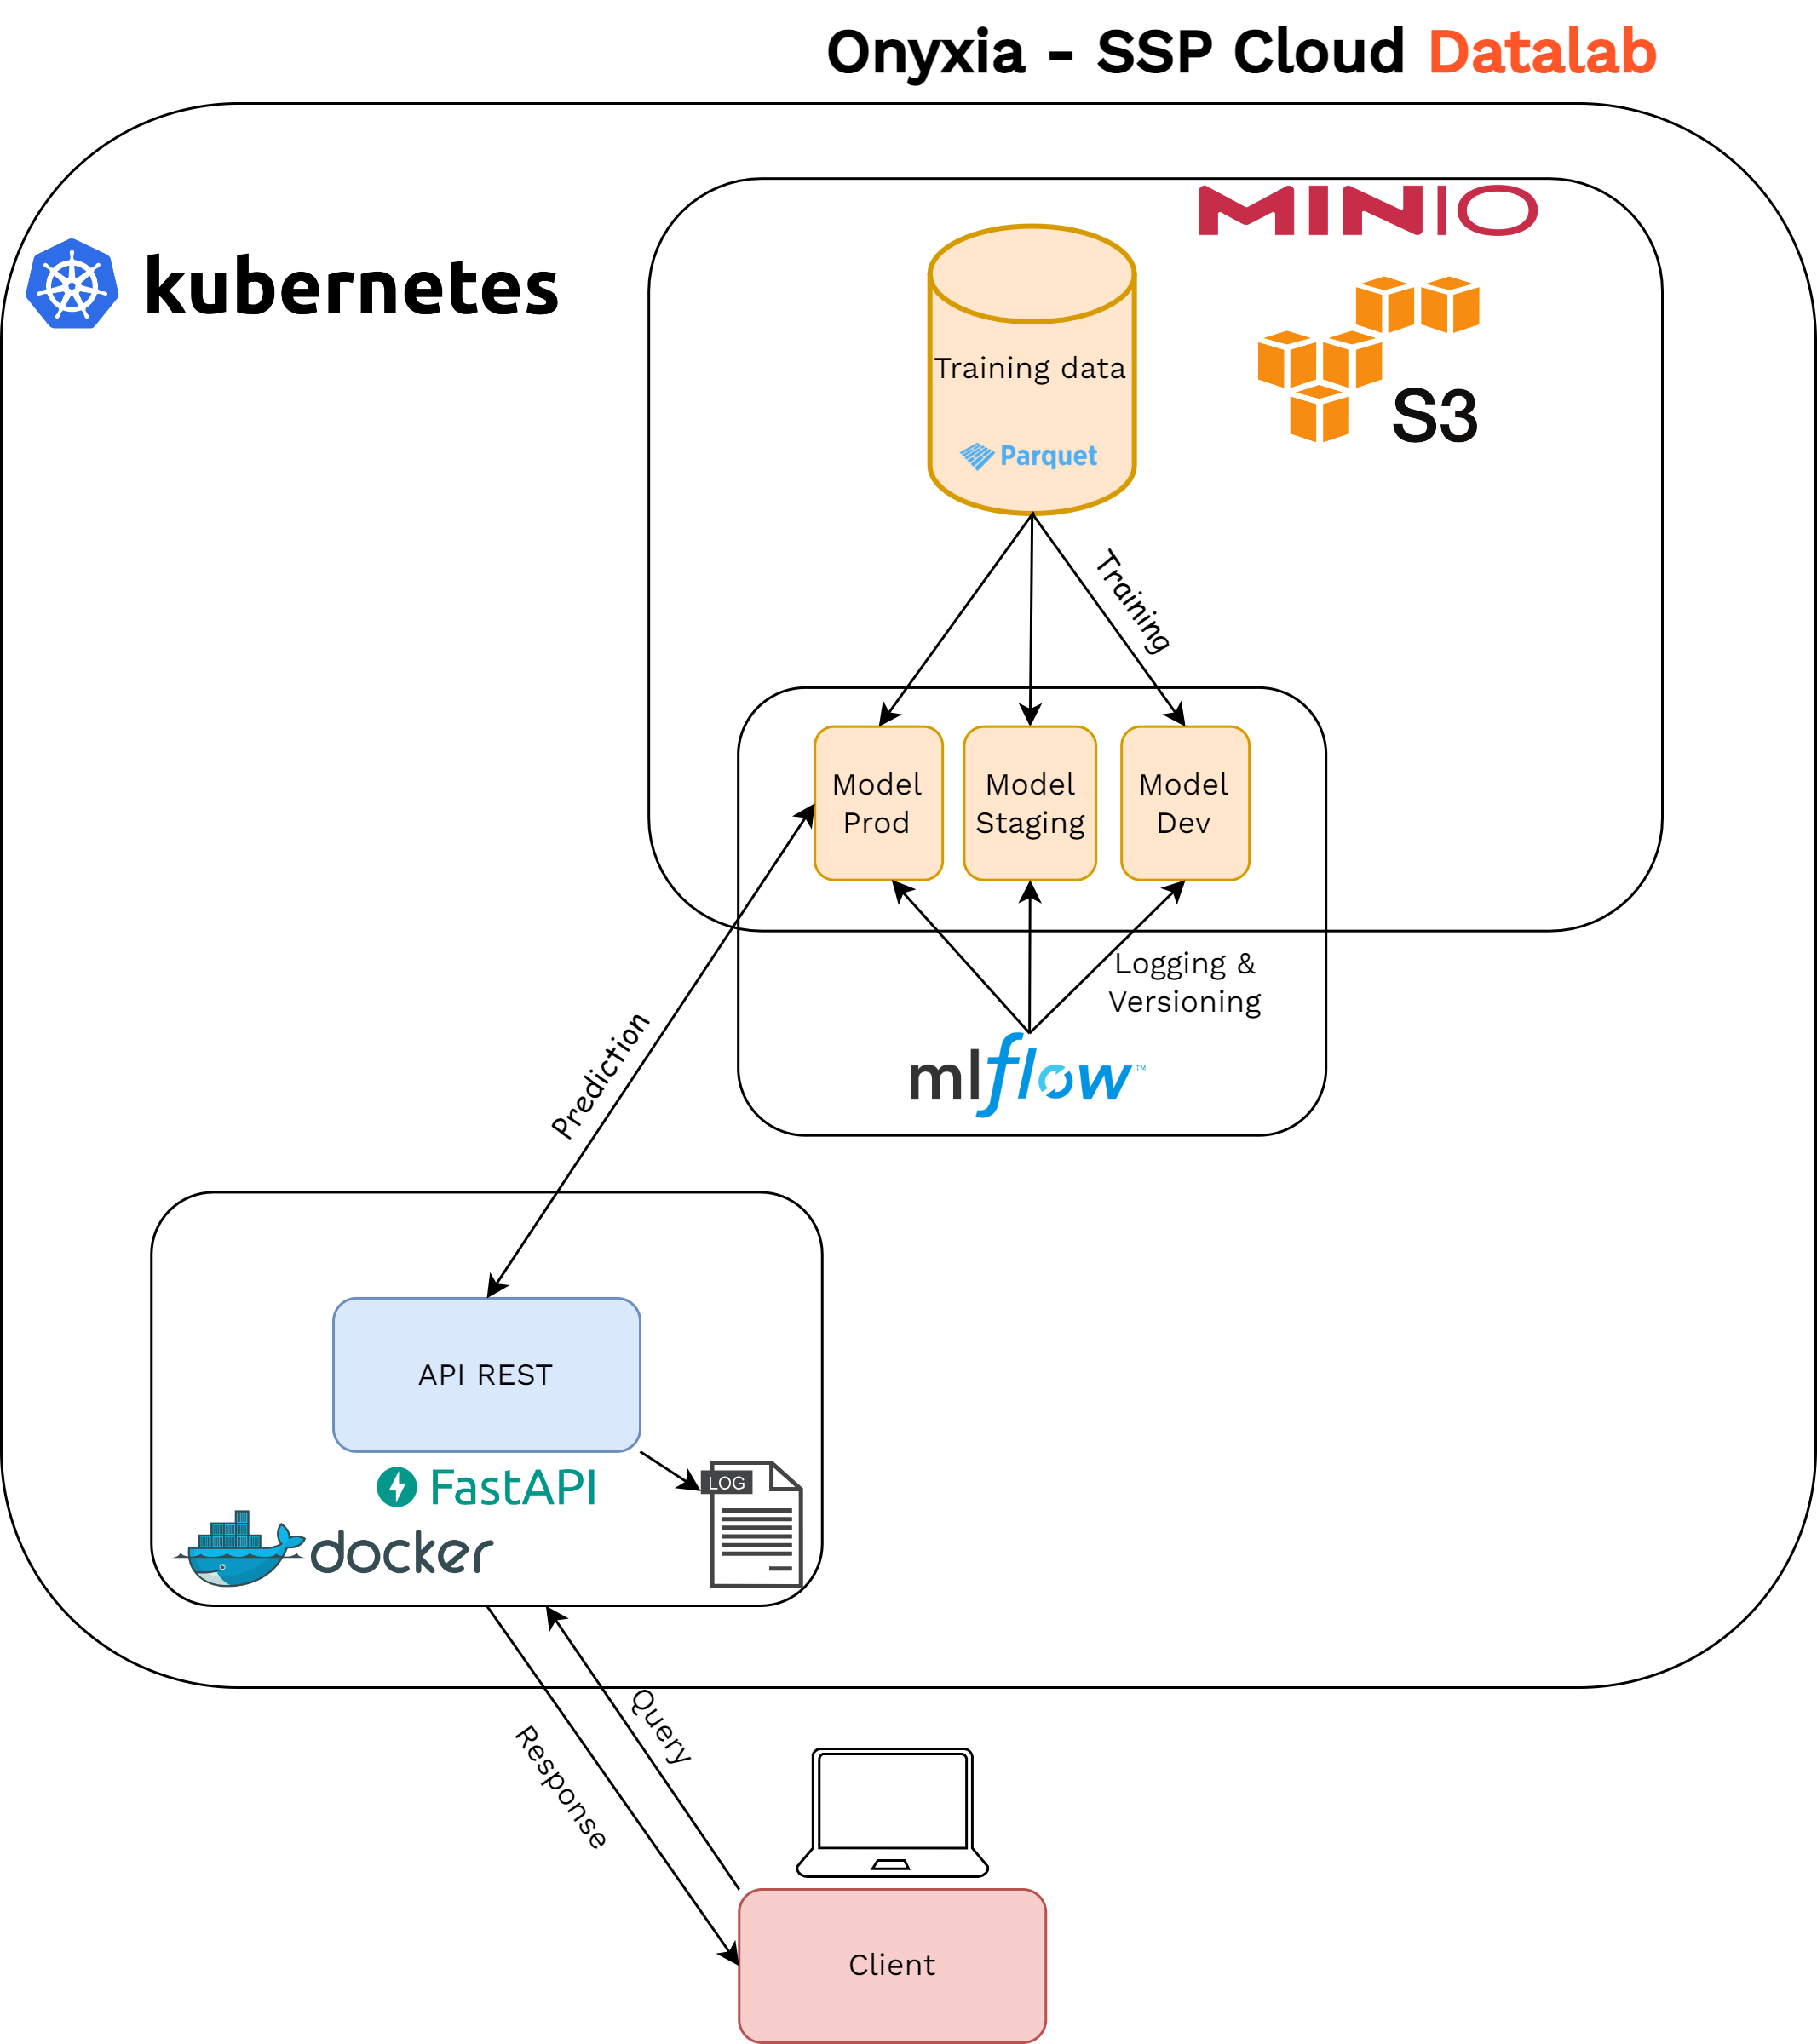
\includegraphics[width=0.75\textwidth]{sections/img/api-datalab.png}}
    \caption{Deploy a ML model via an API}
    \label{fig:api-datalab}
\end{figure}


At this stage, we are already adhering to several MLOps principles in terms of reproducibility through containers and model versioning with MLflow. However, when it comes to automation, there is room for further improvement. Imagine you have deployed an API, and in the meantime, you have developed a new feature for it. For this new feature to be effectively integrated into your API, it is necessary to redeploy the new version of your API and remove the currently deployed one. The idea is to automate the creation of a new Docker image as soon as your API code is updated, and a container based on this latest image automatically deploys the new version of your API. To achieve this on the SSP Cloud, there is the ArgoCD service - CD for Continuous Deployment. ArgoCD continuously scans your Github repository, and as soon as it detects a change in the API code or in the version of the model to be used, it automatically deploys your API by communicating with the Kubernetes cluster. In reality, this process is a bit more nuanced. ArgoCD does not scan your entire repository but only a few configuration files that indicate the versions of the Docker image to use and the model to deploy. To create a new version of the Docker image as soon as the API code is modified, we use the GitHub Actions feature of Github\footnote{An equivalent feature also exists under Gitlab, called Gitlab CI.}. This deployment automation pipeline is depicted in Figure \ref{fig:ci-cd}.

\begin{figure}[htbp]
    \centering
    \makebox[\textwidth][c]{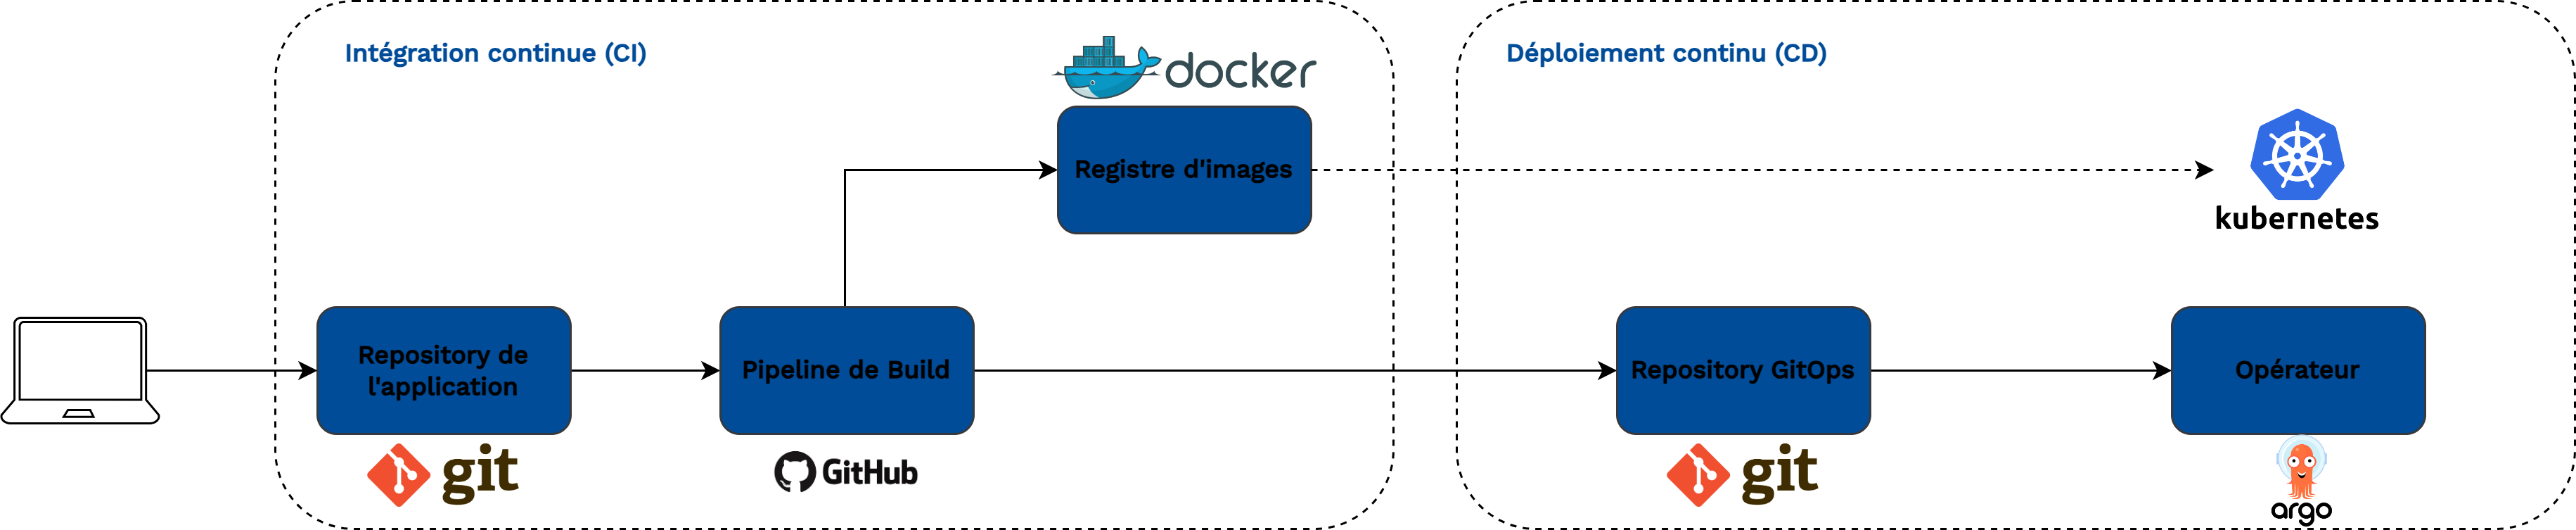
\includegraphics[width=\textwidth]{sections/img/ci-cd.png}}
    \caption{Implementation of CI/CD with Kubernetes}
    \label{fig:ci-cd}
\end{figure}

The autonomy of the data scientist up to the deployment of the model is particularly effective in terms of organization. Indeed, thanks to the deployment of an API or the transmission of a Docker image, transitioning the model to production is facilitated. On the IT side, querying an API is a common task, and no knowledge of ML is required to perform it.

Our MLOps architecture on the SSP Cloud platform was developed incrementally, capitalizing on the platform's modularity. Following the initial deployment of our model, we sought to introduce various enhancements to our architecture, each of which could be integrated independently. This allowed us considerable freedom in selecting our technological solutions. As a result, questions about monitoring the model in its production environment emerged in a subsequent phase.

\subsection{Monitoring of the model}

\subsubsection{The importance monitoring}

Once the modeling phase has been completed, along with training, optimization, and deployment of the model to be accessible to users, it's crucial to understand that the data scientist's responsibilities extend further. Traditionally, the responsibility of the data scientist is often limited to selecting the model to deploy, with the deployment task then delegated to data engineers. However, once in production, the model has not yet reached the end of its lifecycle, and it must be continuously monitored to prevent undesirable performance degradation.

The various components of MLOps, namely data (DataOps), models (ModelOps), and code (DevOps), add complexity to the lifecycle of a ML model by involving multiple stakeholders. Generally, three main actors are involved:

\begin{itemize}
    \item Data scientists/data engineers
    \item IT teams
    \item Business teams
\end{itemize}

Sometimes, data scientists are integrated into business teams and data engineers into IT teams to foster better collaboration. This approach aims to streamline skills, unify terminologies, and align project objectives. In any cases, effective communication remains essential to ensure proper management of the lifecycle of a ML model, particularly concerning monitoring its behavior in a production environment. Continuous monitoring of the deployed model is extremely important to ensure the conformity of results to expectations, anticipate changes in data, and iteratively improve the model. The monitoring is a crucial element of the MLOps approach.

The concept of monitoring can take on different meanings depending on the context of the involved team. For IT teams, it primarily involves verifying the technical validity of the application, including aspects such as latency, memory consumption, or disk usage. Conversely, for data scientists or business teams, the focus is more on methodological monitoring of the model. However, real-time tracking of the performance of a ML model is often a complex task, given that ground truth is usually not known at the time of prediction. Therefore, it is common to use proxies to detect any signs of performance degradation. Two main types of degradation of a ML model are generally distinguished: data drift and concept drift.

\begin{itemize}
    \item \textbf{Data drift}: Data drift occurs when the data used during inference in production exhibits significant differences compared to the data used during training, that is,  $\mathds{P}_{train}(X) \neq \mathds{P}_{inference}(X)$.
    \item \textbf{Concept drift}: Concept drift is evoked when a change in the statistical relationship between the features ($X$) and the target variable ($Y$) is observed over time, that is, $\mathds{P}_{train}(Y|X) \neq \mathds{P}_{inference}(Y|X)$ and $\mathds{P}_{train}(X) = \mathds{P}_{inference}(X)$.
\end{itemize}


\subsubsection{What do we monitor ?}

In our use case, our objective is to achieve the highest number of correctly classified textual description while minimizing the number of textual description requiring manual intervention. Thus, our goal is to distinguish correct predictions from incorrect ones without prior access to ground truth. To accomplish this, we have developed a confidence index, which represents the difference between the two highest scores. Therefore, for a given textual description, if the confidence index exceeds a determined threshold, the textual description is automatically coded. Otherwise, the textual description is manually coded by an Insee's agent who has access to the five most probable codes according to the model to optimize manual intervention. Defining the threshold for automatic coding of textual descriptions is crucial in production deployment. It involves making trade-offs between achieving a high automatic coding rate and preserving model performance, and vice versa.

To monitor the behavior of our model in production, we have developed an interactive dashboard that enables visualization of several metrics of interest for the business teams. Among these metrics are the number of requests per day and the rate of automatic coding per day based on a given confidence index threshold. This visualization allows business teams to understand the rate of automatic coding they would have obtained if they had chosen different thresholds. It is also possible to visualize the distribution of obtained confidence indices and to compare two temporal windows to determine if there are changes in the distributions of predictions returned by the model\footnote{To compare distributions, you need to calculate the distances between them using, for example the \href{https://en.wikipedia.org/wiki/Bhattacharyya_distance}{Bhattacharyya distance}, the \href{https://en.wikipedia.org/wiki/Kullback\%E2\%80\%93Leibler_divergence}{Kullback-Leibler divergence}, the \href{https://en.wikipedia.org/wiki/Hellinger_distance}{Hellinger distance} or to perform statistical tests such as the \href{https://en.wikipedia.org/wiki/Kolmogorov\%E2\%80\%93Smirnov_test}{Kolmogorov–Smirnov test}, or the \href{https://en.wikipedia.org/wiki/Chi-squared_test}{$\chi^2$-test}.}. 

Confidence indices can be analyzed at finer levels of granularity based on the aggregation level of the nomenclature, to determine which classes are most difficult to predict and which have more or less occurrences. Another part of the dashboard focuses more on the input data of the model and details, for example, the average number of words per textual description, the average number of sentences per textual description, as well as the most frequent words, etc.

\subsubsection{How to implement a monitoring system in the SSP Cloud?}

Although there are several solutions for monitoring ML models such as \href{https://www.evidentlyai.com/}{Evidently} or \href{https://www.siffletdata.com/}{Sifflet}, we preferred to implement our own solution. Indeed, at the time of our trials, none of the open-source solutions available on the market seemed optimal to us. However, the field of monitoring ML models is still emerging and actively developing, so the statements made today may no longer be true at the time of reading these lines. Before opting, as we did, for an internal solution, we recommend exploring the available tools first.

In our case, we chose to use tools that we already mastered and that seemed suitable for our problem. We thus used DuckDB for optimized management of our data and the Dashboard feature of Quarto for creating the interactive dashboard. 

First, to monitor in real-time the activities of your API, it is essential to integrate logs, whether to monitor technical or methodological aspects. We made the decision, which may be subject to debate, to include \textit{business information} such as the output code and its corresponding confidence index in the API logs. The objective was to be able to build our dashboard based on the logs returned by the API. To exploit these logs, we set up a kind of Extract-Transform-Load (ETL) process in Python, which retrieves the API logs and transforms them into partitioned parquet files exploitable by the dashboard. Ideally, we would have preferred to rely on a tool capable of performing this parsing natively and more structured than us. \href{https://www.parseable.com/}{Parseable} could have been such a solution, but unfortunately, it was not installable on the SSP Cloud for technical reasons. We then use Quarto and its Dashboard feature to create an interactive dashboard. The various metrics present in the dashboard are calculated by making SQL queries directly on our parquet files with DuckDB. The dashboard is deployed in the same way as our API, that is, in a container based on an image that is automatically built via Github Actions as soon as the code associated with the dashboard is modified. Figure \ref{fig:monitoring-datalab} depicts the setup of our monitoring system, highlighting the various technologies employed.

In summary, our monitoring pipeline consists of:

\begin{enumerate}
    \item Including \textit{business logs} in the API for every request.
    \item Utilizing ArgoCD to schedule a nightly ETL job, generating partitioned parquet files stored on MinIO.
    \item Employing ArgoCD for continuous deployment, where the dashboard dynamically retrieves data from the parquet file via DuckDB, computes metrics, and offers interactive visualization.

\end{enumerate}

\begin{figure}[htbp]
    \centering
    \makebox[\textwidth][c]{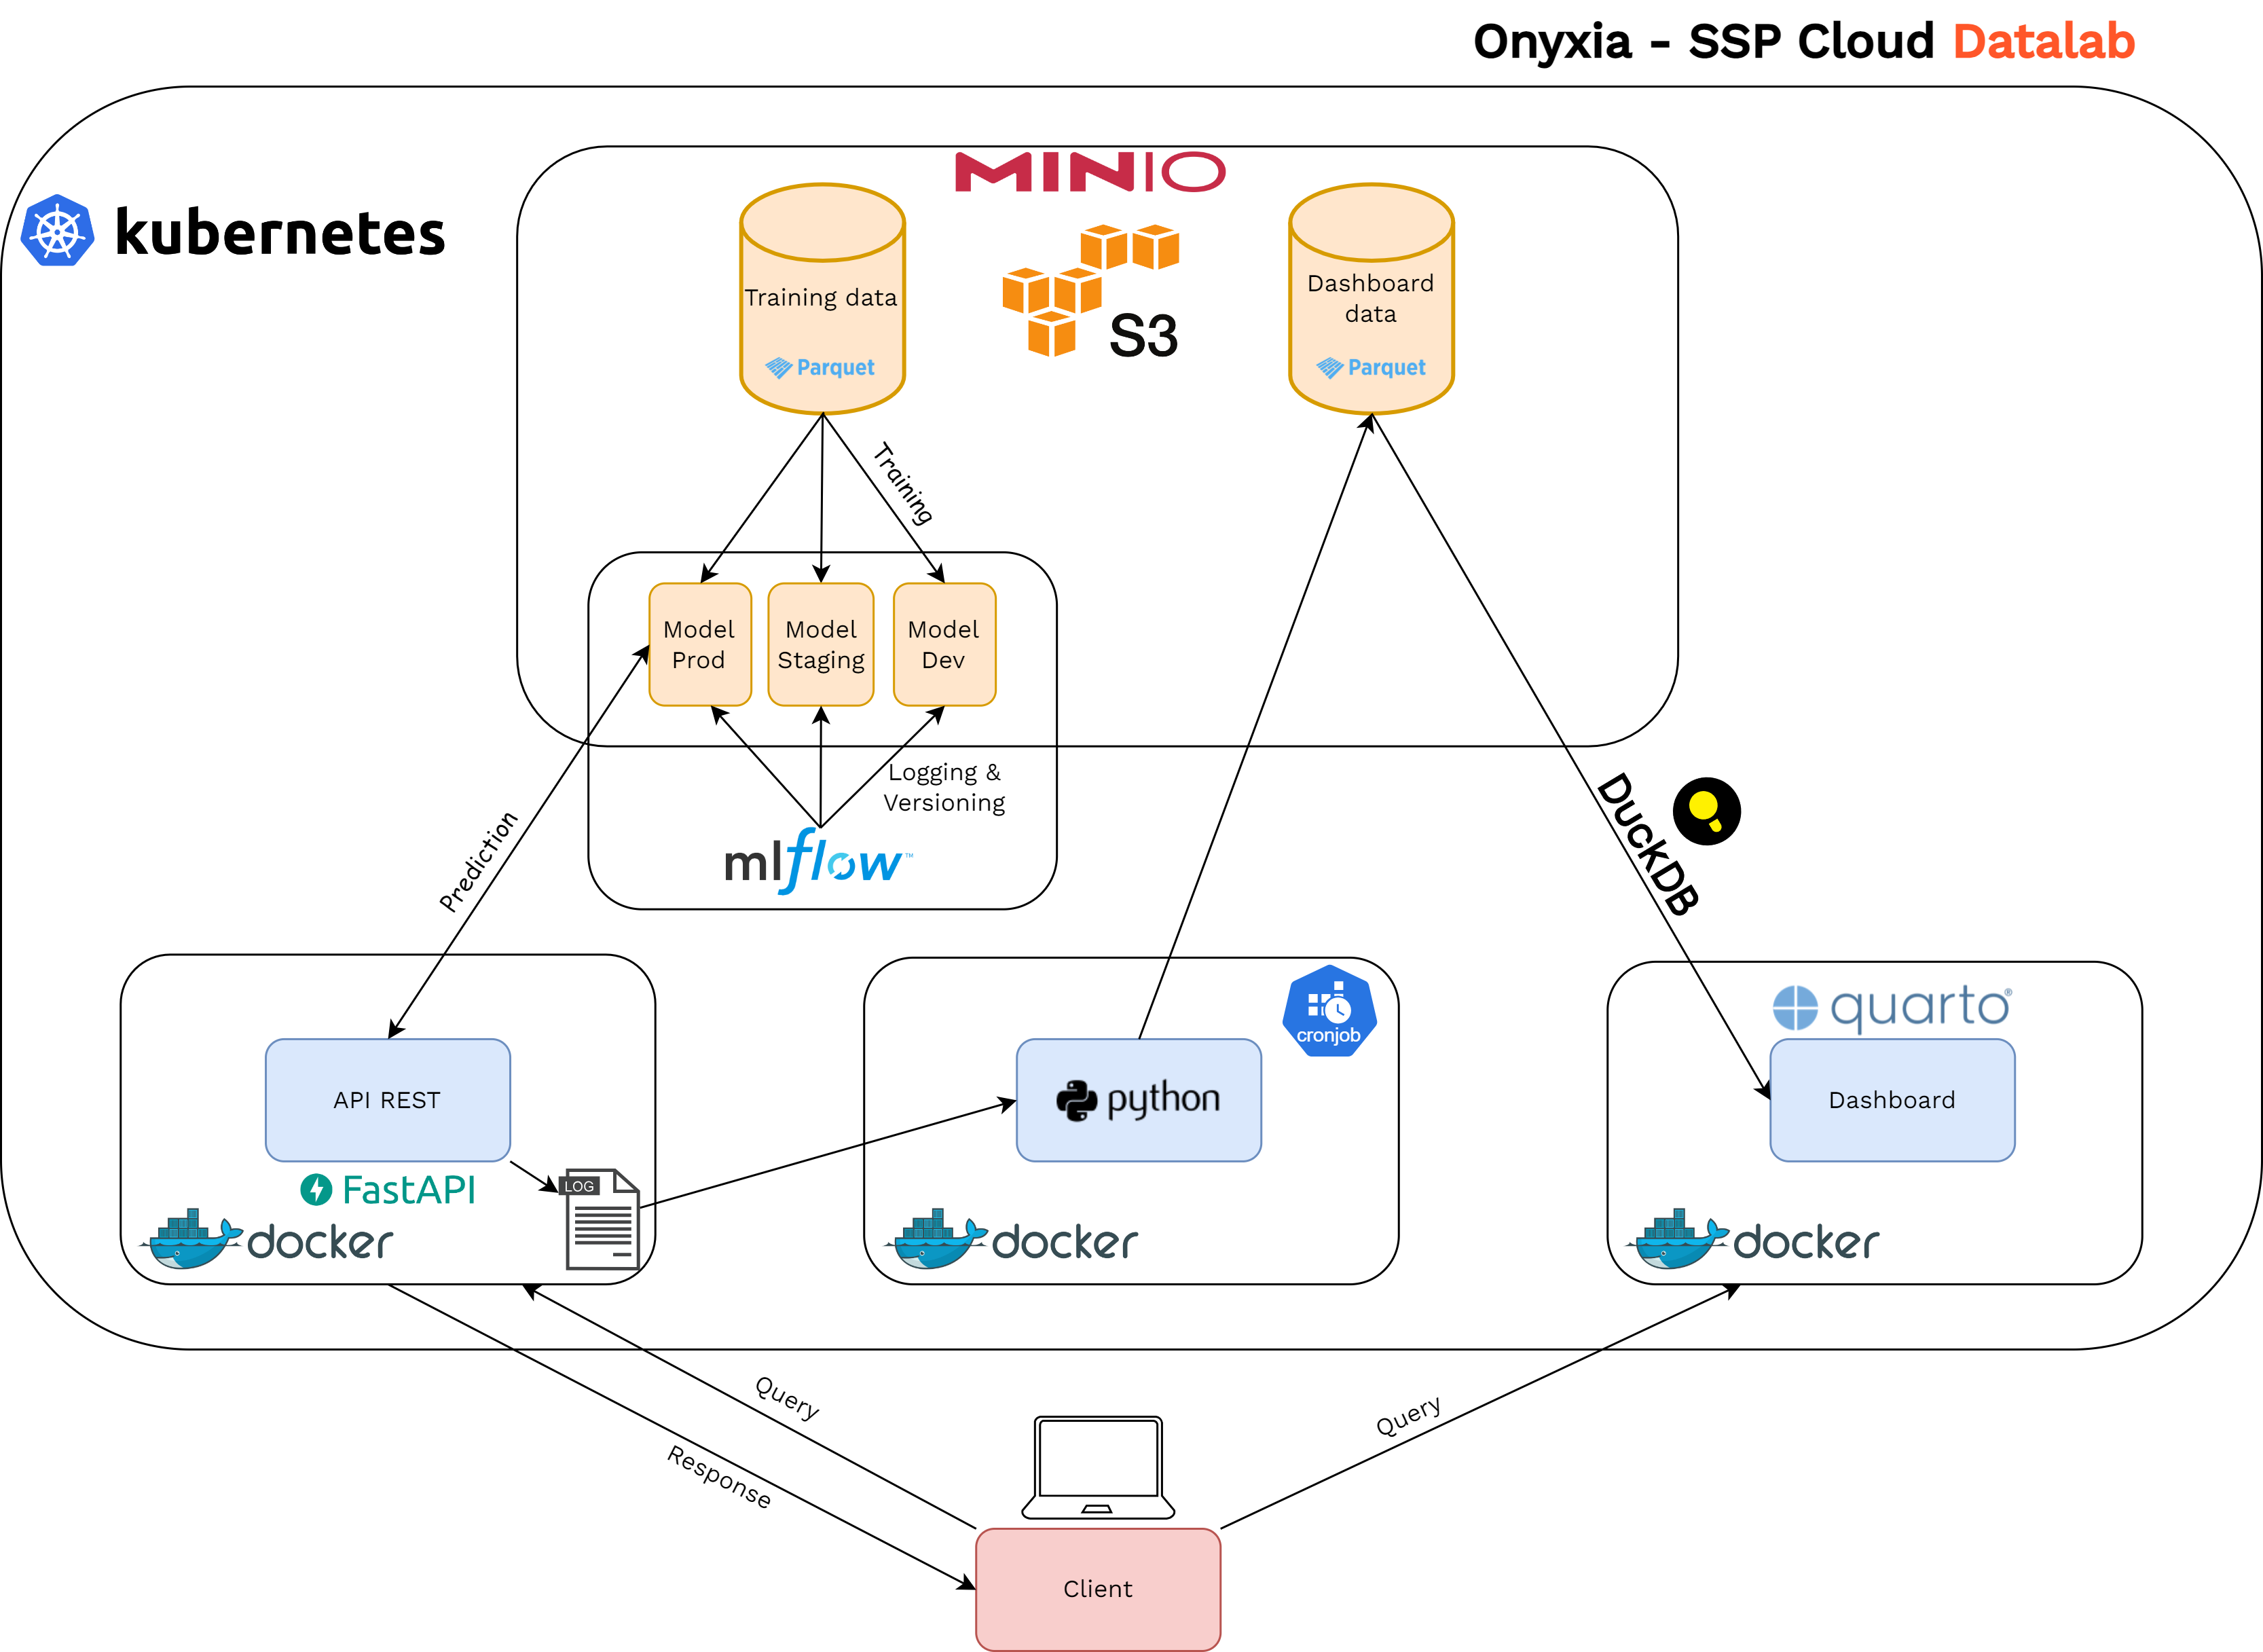
\includegraphics[width=1.5\textwidth]{sections/img/monitoring-datalab.png}}
    \caption{TODO}
    \label{fig:monitoring-datalab}
\end{figure}


\subsection{Continuous Annotation}

In all ML projects, it is well-established that data is key, and in supervised ML problems, annotations play a crucial role in model performance. At the project's onset, time constraints compelled us to swiftly achieve results, precluding the luxury of conducting a comprehensive annotation campaign. Consequently, we never had access to a truly annotated gold-standard test sample on which we could rely 100\%. To evaluate the performance of our model, we relied on a subset of our training dataset (test/train split), knowing that its labeling was not perfect. After several months of model deployment, it became imperative to build such a gold-standard test sample. Firstly, this sample allows us to have an unbiased view of the model's performance in production on real data, particularly on data that has been automatically coded. Additionally, this sample enabled us to identify and correct inconsistencies present in our initial training dataset. 

Convincing the business teams of the significance of annotation proved challenging, as they were reluctant to reallocate new human resources, which necessitated specialized expertise, on a tedious task. However, the model's increased automation in coding enabled the teams to shift their focus to annotation tasks.


Another reason that motivated the implementation of annotation campaigns is the redesign of the NACE nomenclature in 2025. From 2025 onwards, European statistical institutes will be required to use the latest version of NACE, namely NACE Rev. 2.1. This revision brings substantial changes that will require retraining a new model. For this, a new training dataset with the correct annotations is peremptory. A back-propagation work on the old training dataset is also considered to increase the size of the dataset. Thus, a dual annotation campaign was initiated in early 2024 on the SSP Cloud platform.

To carry out these annotation campaigns, we used the \href{https://labelstud.io/}{Label Studio} service, available on the SSP Cloud. Label Studio is an open-source platform designed to facilitate data annotation. The first annotation campaign aims to create a test dataset allowing continuous evaluation of our model and improvement of the training dataset if necessary. To do this, we create a pool of text descriptions randomly sampled from the data passed through the API over the past three months. This sample is then sent to annotation by NACE experts using the UI of Label Studio. The annotation results are automatically saved on MinIO, transformed into parquet format, and then integrated into the monitoring dashboard to compute and observe various model performance metrics. The second annotation campaign is dedicated to the transition to the new version of NACE. The objective is to allocate certain experts to annotation in the new version of NACE to create a training dataset for the future model. In this revision, some codes are univocal, meaning for example that code 0112Z will become 0112Y, while others are multivocal, such as 0119Z, which can become either 0113Y or 0119Y. The challenge lies primarily with the latter, which is why, to streamline this annotation process, only the textual descriptions of multivocal codes are sent for annotation on Label Studio.

Once again, the presence of a cloud-native technology on the platform, such as Label Studio, allowed us to swiftly kickstart this annotation campaign while seamlessly integrating it with the various components of our architecture, as depicted in Figure \ref{fig:annotation-datalab}.

\begin{figure}[htbp]
    \centering
    \makebox[\textwidth][c]{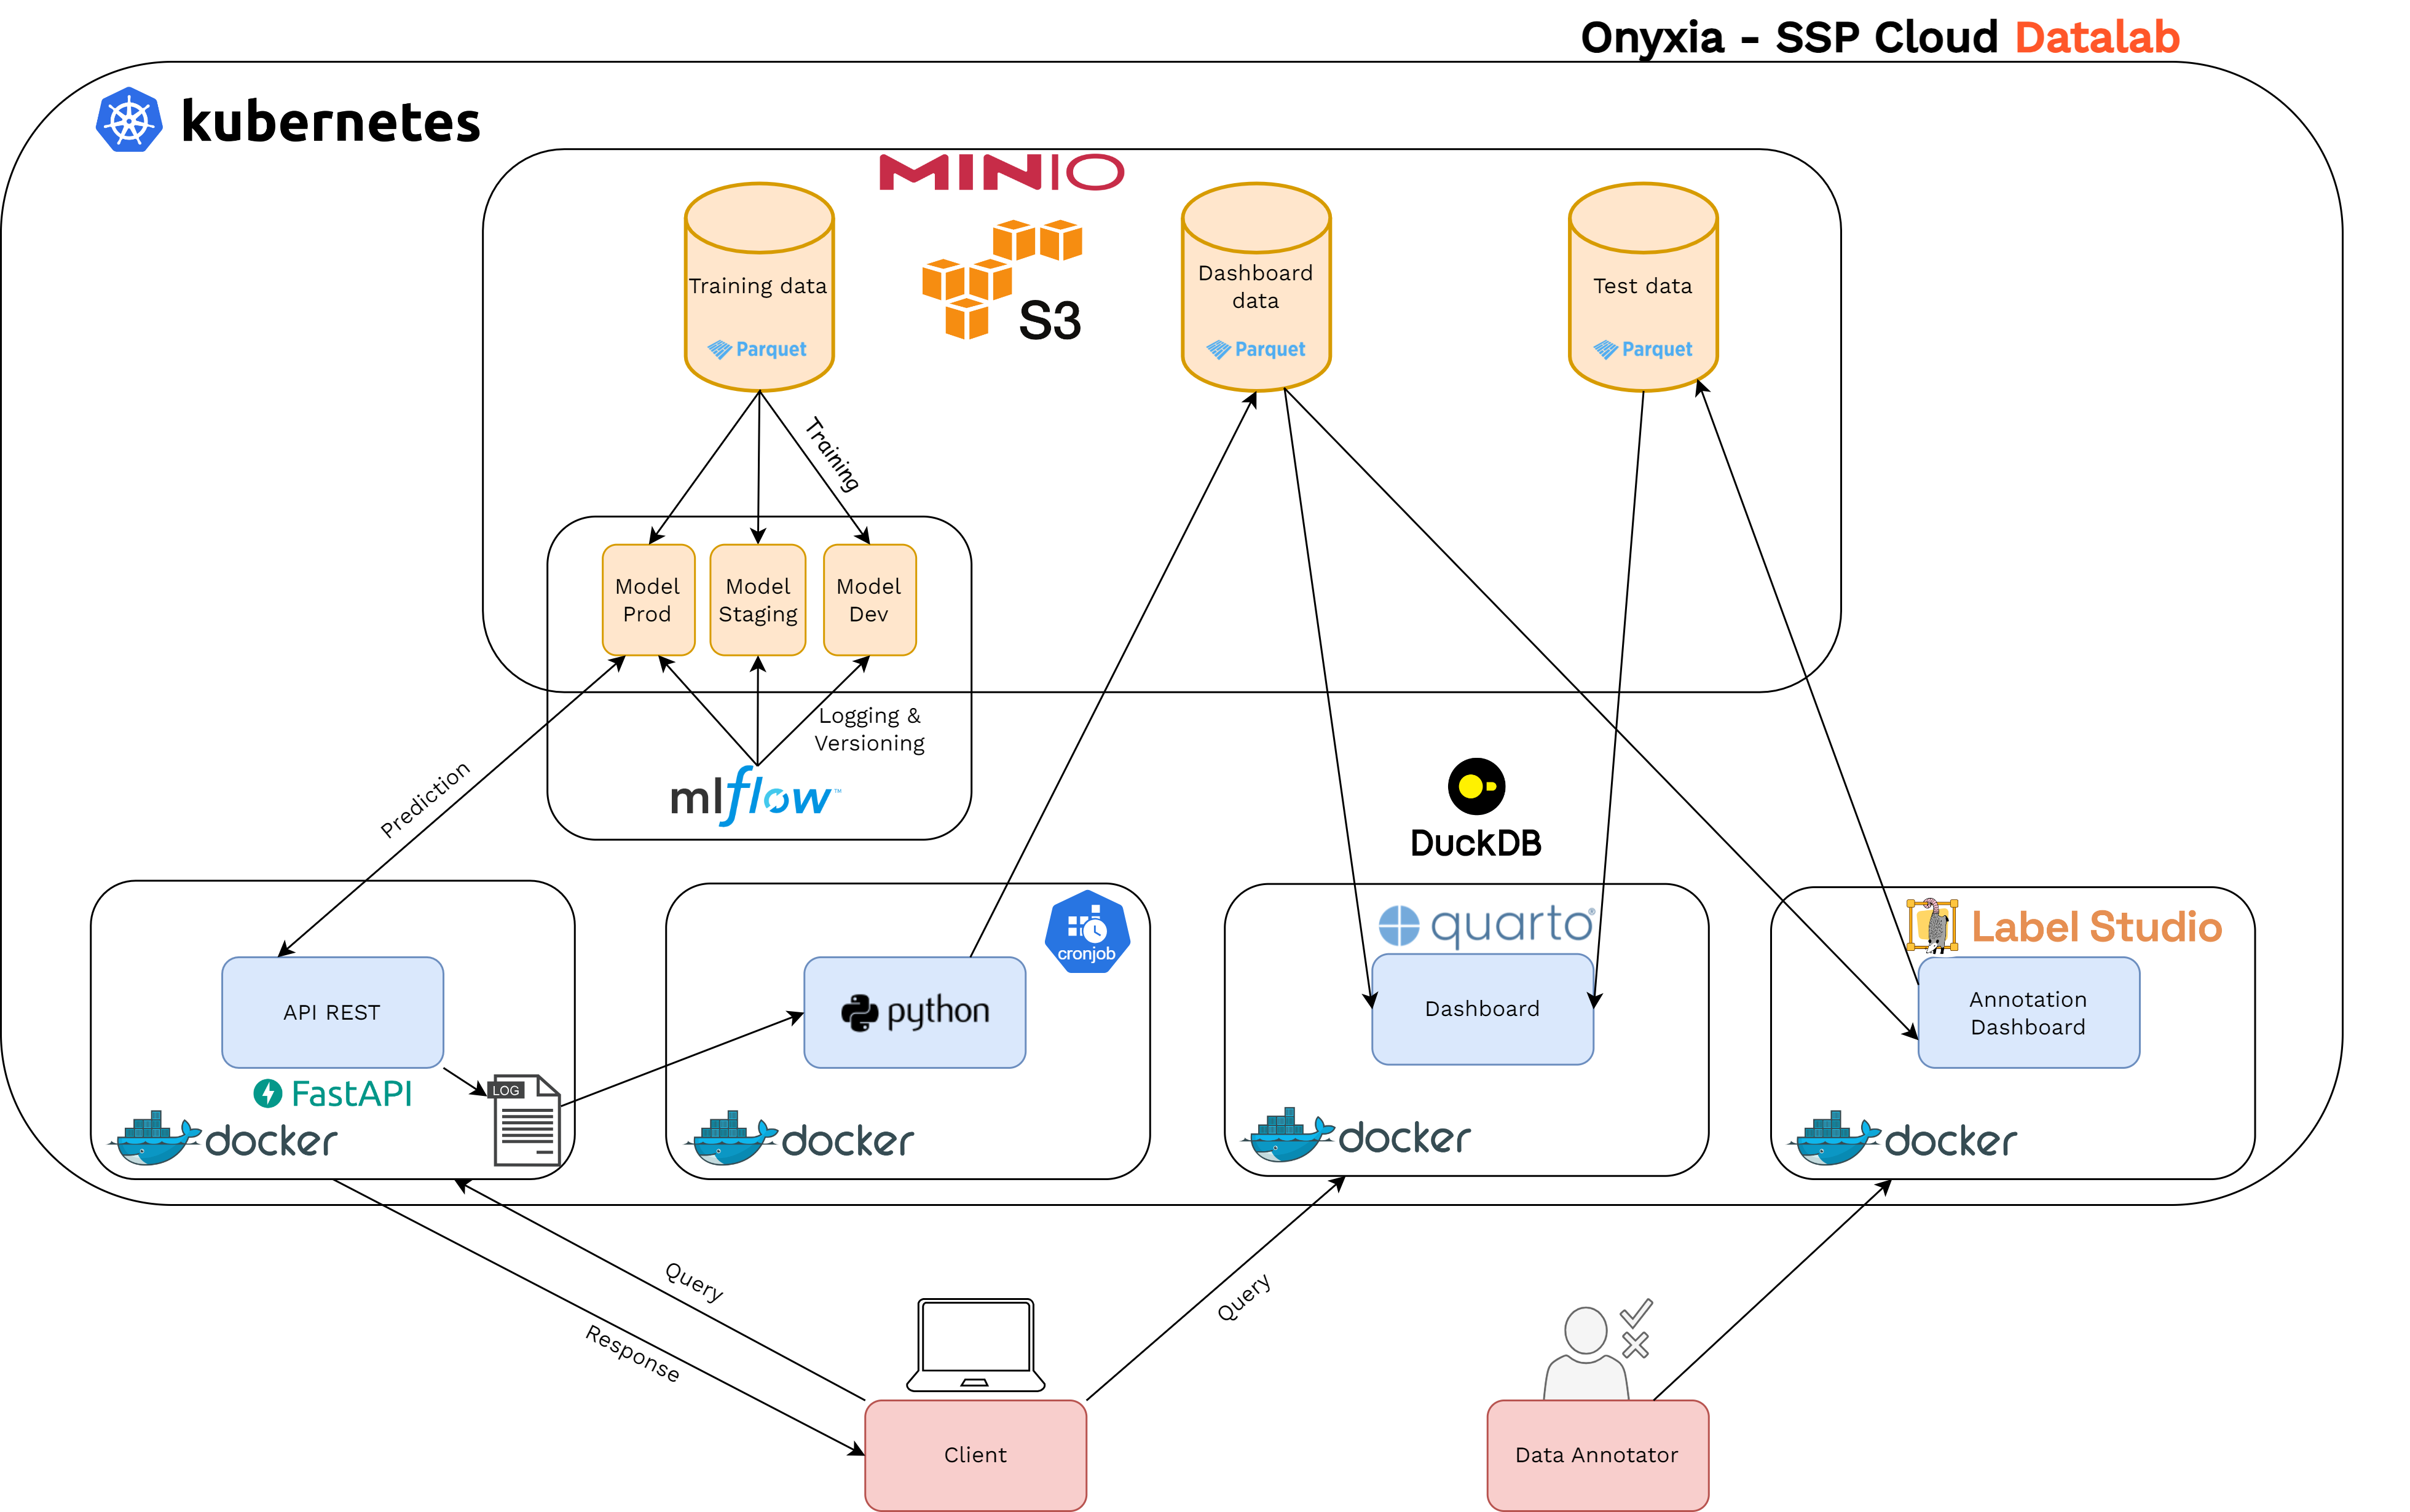
\includegraphics[width=1.5\textwidth]{sections/img/annotation-datalab.png}}
    \caption{TODO}
    \label{fig:annotation-datalab}
\end{figure}

\subsection{What next ?}

We believe that a well-designed infrastructure facilitates the adoption of MLOps principles across all stages of an ML project, automating a multitude of tasks. The SSP Cloud stands out as a fitting illustration of this concept.
An important aspect of MLOps is its iterative nature: not all components can be fully integrated from the outset, and time limitations can be constraining. There are several maturity level of MLOps. Therefore, it's advisable to begin by establishing robust development practices and gradually enriching the project with increased automation as requirements evolve. An effective initial step is to leverage tools like MLflow, which facilitate adherence to the MLOps framework.

We've identified various areas where we can improve our processes, which we plan to address in the near term. Our primary focus will be on automating model retraining, although this will require enhancements to our monitoring pipeline. Despite the availability of a dashboard for business teams to visualize the model's performance almost in real-time (updated nightly), we currently lack an alert system to signal when retraining is required, and there's an even more ambitious goal of automating this retraining process.


Additionally, we plan to test other methodologies for our model, especially Transformer-type models, which could soon be usable on our production servers. Finally, although this does not directly optimize our pipeline in terms of MLOps, working on the revision of NACE will be an interesting challenge and will allow us to assess the relevance of the MLOps approach we have adopted since the beginning of the project.
